\subsection{Efficienza locale}

Utilizzando gli stessi dati della \autoref{attenu}, abbiamo studiato le variazioni di efficienza in vari punti del PM1. In \autoref{capolavoro} è presente un grafico 3D che mostra i conteggi ottenuti in ogni casella in cui è stato posizionato il miniscint. Si può apprezzare una diminuzione dei conteggi tra le varie colonne per i motivi discussi in \autoref{attenu} ma è anche evidente come all'interno di una stessa colonna ci siano delle variazioni significative tra una riga e l'altra.
\marginpar{Non so cosa scrivere. Se lo sapete scrivetelo. Io intanto lavoro su altro.}
\begin{figure}[h]
\flushleft
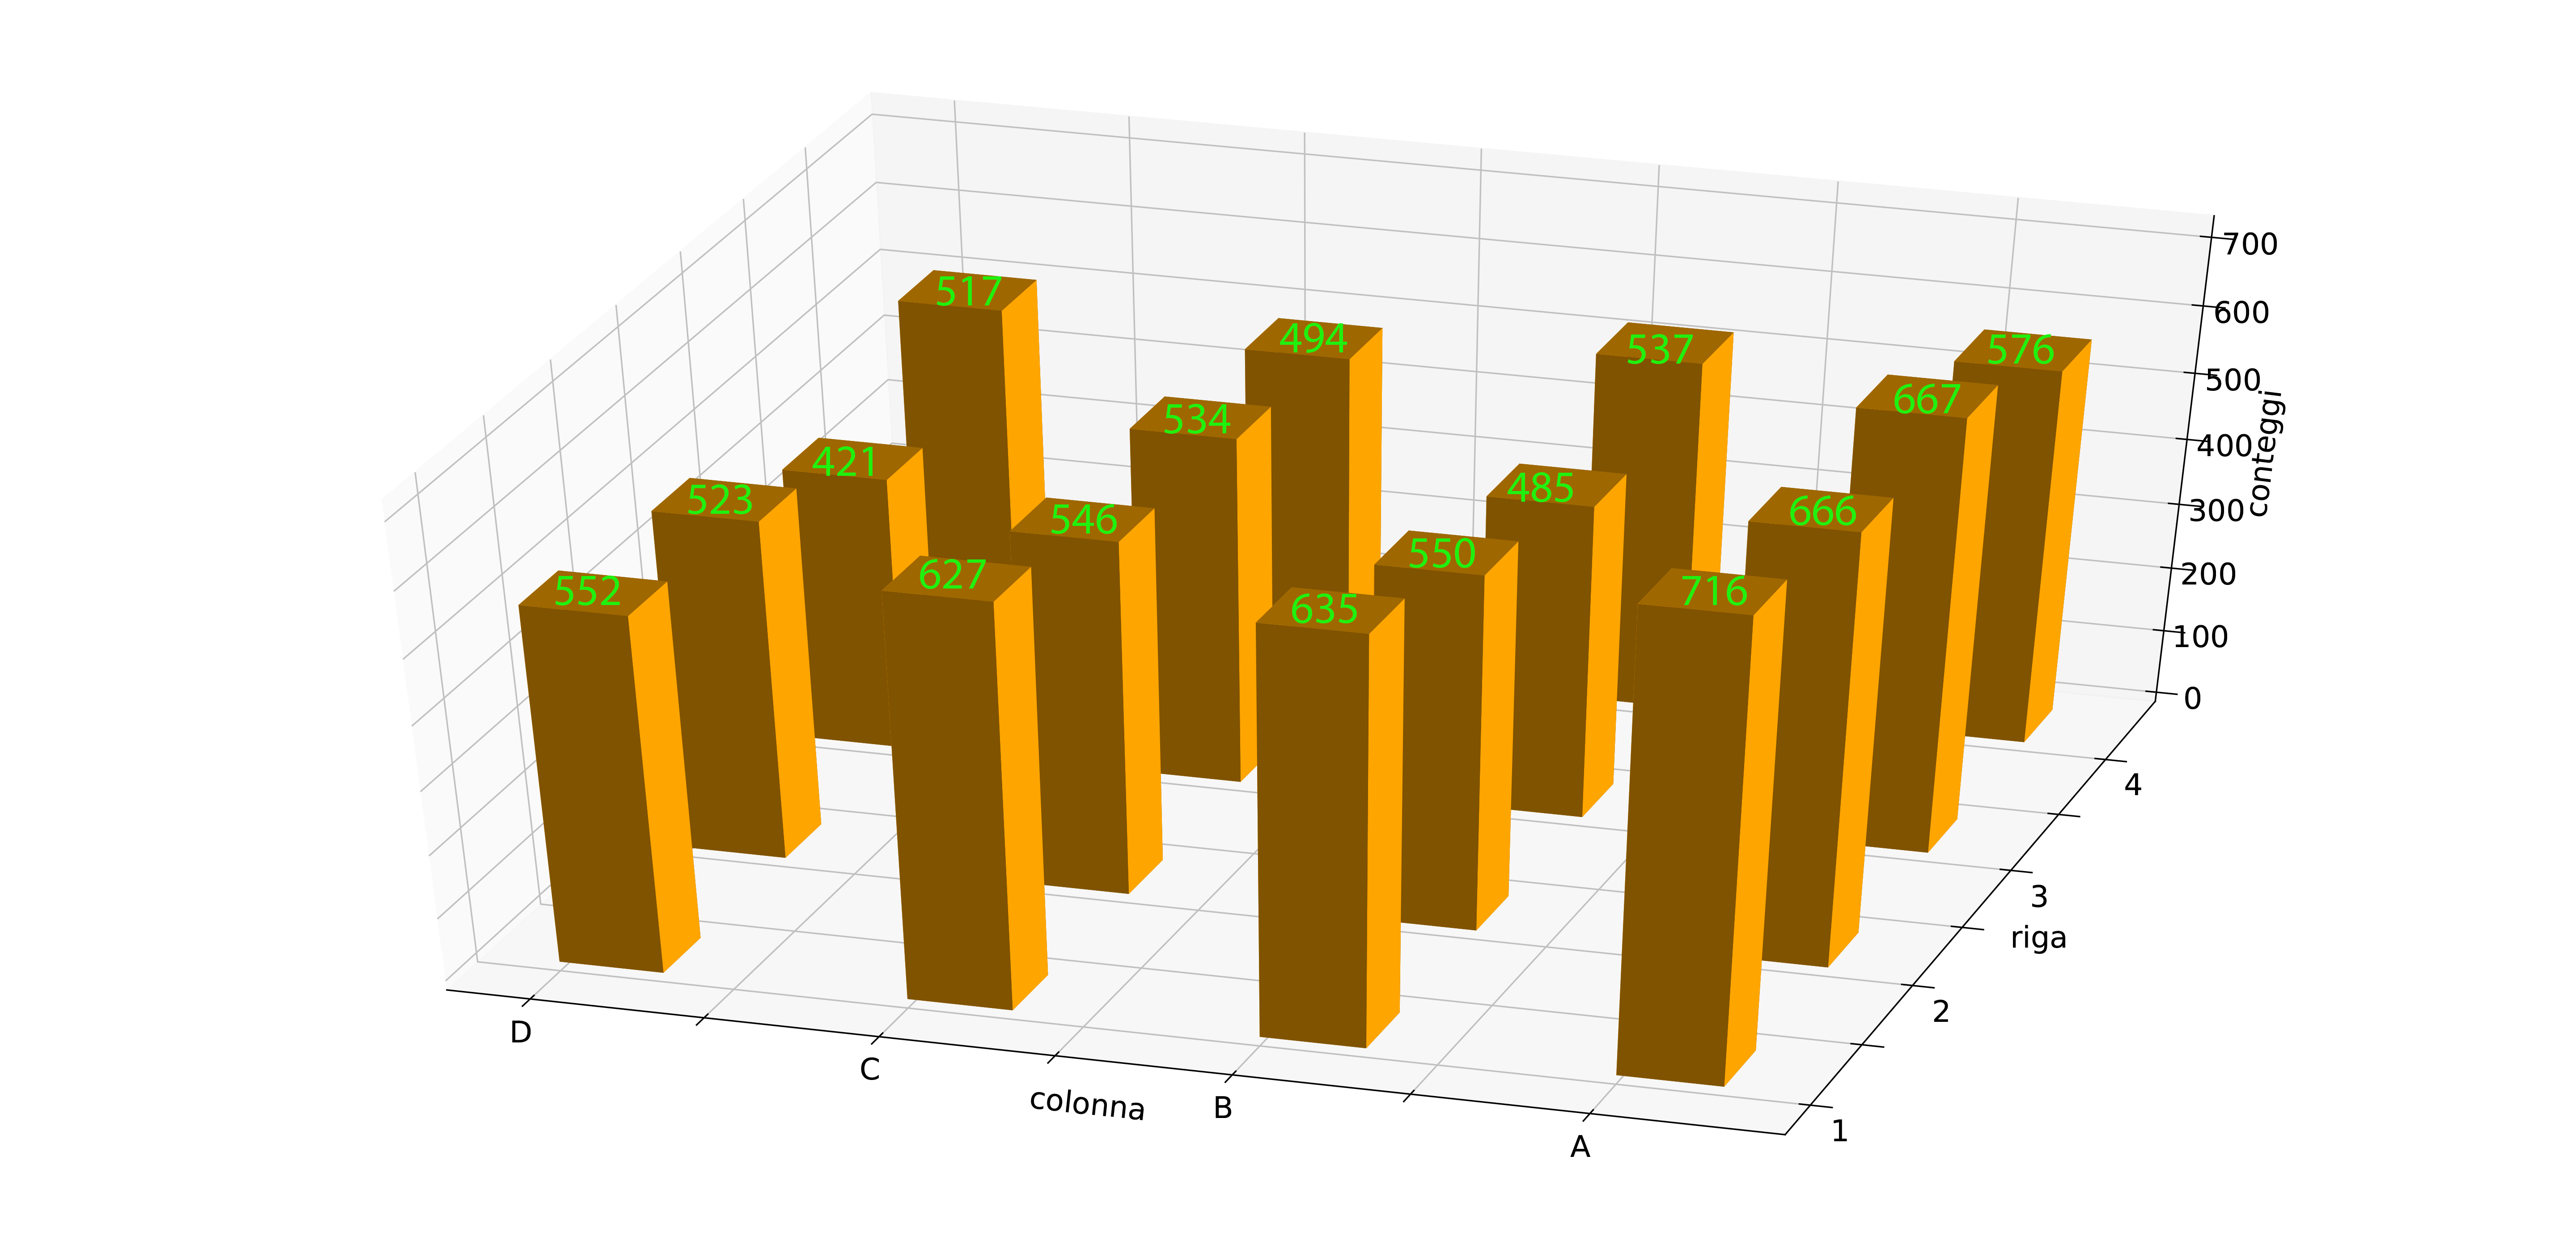
\includegraphics[width=17 cm]{3d_rit}
\caption{Conteggi PM1 nelle rispettive caselle. L'errore su ogni conteggio è la radice quadrata dello stesso. La disposizione delle caselle è la stessa che in quel disegno che Jack farà perché è bravo a disegnare anche al computer.}
\label{capolavoro}
\end{figure}

